\documentclass{article}

\usepackage[english]{babel}
\usepackage[utf8]{inputenc}
\usepackage[T1]{fontenc}
\usepackage{amsmath, amsfonts, amssymb, amsthm}
\usepackage{tikz}
\usepackage{csquotes}
\usepackage{stmaryrd}


\usepackage[backend=biber,citetracker=true]{biblatex}
\addbibresource{bibli.bib}
\usepackage{color}
\usepackage{subcaption}
\usepackage{graphicx}
\usepackage{./tex/sty/scribe}
\usepackage{float}


%\usepackage{epsfig}
%\usepackage{ulem, stmaryrd, dsfont}


\author{Fanchon Herman}


\begin{document}
\begin{titlepage} 
	\newcommand{\HRule}{\rule{\linewidth}{0.5mm}}
	
	\center
	
	\textsc{\LARGE University of Montpellier}\\[1.5cm]
	
	\textsc{\Large Master 2 Biostatistics }\\[0.5cm] 
	
	\textsc{\large HMMA$308$ Project}\\[0.5cm] 

	\HRule\\[0.4cm]
	
	{\huge\bfseries Recommendation system}\\[0.4cm] 
	
	\HRule\\[1.5cm]
	
	\begin{minipage}{0.4\textwidth}
		\begin{flushleft}
			\large
			\textit{Student: }\\
			Fanchon Herman
		\end{flushleft}
	\end{minipage}
	~
	\begin{minipage}{0.4\textwidth}
		\begin{flushright}
			\large
			\textit{Teacher: }\\
			Joseph Salmon\\
		\end{flushright}
	\end{minipage}
		\vfill 
	
	{\large 2020-2021} 

		\vfill\vfill
		
\centering

\includegraphics[width=0.2\textwidth]{./images/Logo}


	
	 
	%----------------------------------------------------------------------------------------
	
	\vfill 
\end{titlepage}

\tableofcontents
\newpage
%%%%%%%%%%%%%%%%%%%%%%%%%%%%%%%%%%%%%%%%%%%%%%%%%%%%%%%%%%%%%%%%%%%%%%%%%%%%%%%
%%%%%%%%%%%%%%%%%%%%%%%%%%%%%%%%%%%%%%%%%%%%%%%%%%%%%%%%%%%%%%%%%%%%%%%%%%%%%%%
\section*{Introduction}

The aim of this project is to automatically predict the notes that a user will give to a film or music that he does not yet know. The database used throughout this project is MovieLens (100k).
First, we will explain the dataset in order to know more about it. Then, we will study the sparsity of a particular matrix to finally use the matrix factorization in order to allow to reduce the dimensions.
%%%%%%%%%%%%%%%%%%%%%%%%%%%%%%%%%%%%%%%%%%%%%%%%%%%%%%%%%%%%%%%%%%%%%%%%%%%%%%%
%%%%%%%%%%%%%%%%%%%%%%%%%%%%%%%%%%%%%%%%%%%%%%%%%%%%%%%%%%%%%%%%%%%%%%%%%%%%%%%

%%%%%%%%%%%%%%%%%%%%%%%%%%%%%%%%%%%%%%%%%%%%%%%%%%%%%%%%%%%%%%%%%%%%%%%%%%%%%%%
%%%%%%%%%%%%%%%%%%%%%%%%%%%%%%%%%%%%%%%%%%%%%%%%%%%%%%%%%%%%%%%%%%%%%%%%%%%%%%%
\section{Data presentation}
The MovieLens (100k) database was collected by the GroupLens research project at the University of Minnesota. It includes:
\begin{itemize}
    \item $100,000$ ratings of $943$ users on $1682$ movies (between $1$ and $5$),
    \item each user has evaluated at least $20$ films,
    \item simple demographic information for users.
\end{itemize}

\begin{center}
    \begin{tabular}{|c|c|c|c|c|c|}
    \hline
         & user ID & movie ID & rating & timestamp \\
         \hline \hline
         0 & 196 & 242 & 3 & 881250949\\
         1 & 186 & 302 & 3 & 891717742\\
         2 & 22 & 377 & 1 & 878887116\\
         3 & 244 & 51 & 2 & 880606923\\
         \hline
    \end{tabular}
    \captionof{table}{Extraction of some data.} 
\end{center}

In view of the dataset, we can represent some visualizations in order to see more clearly.
The first wise thing to do is to convert the timestamp in order to get the year and month the user has noted the movie  seen.
We can ask ourselves how the ratings are distributed but also the number of ratings posted per month. Let’s see these results below.

\begin{figure}[H]
\centering
\begin{subfigure}{.5\textwidth}
  \centering
  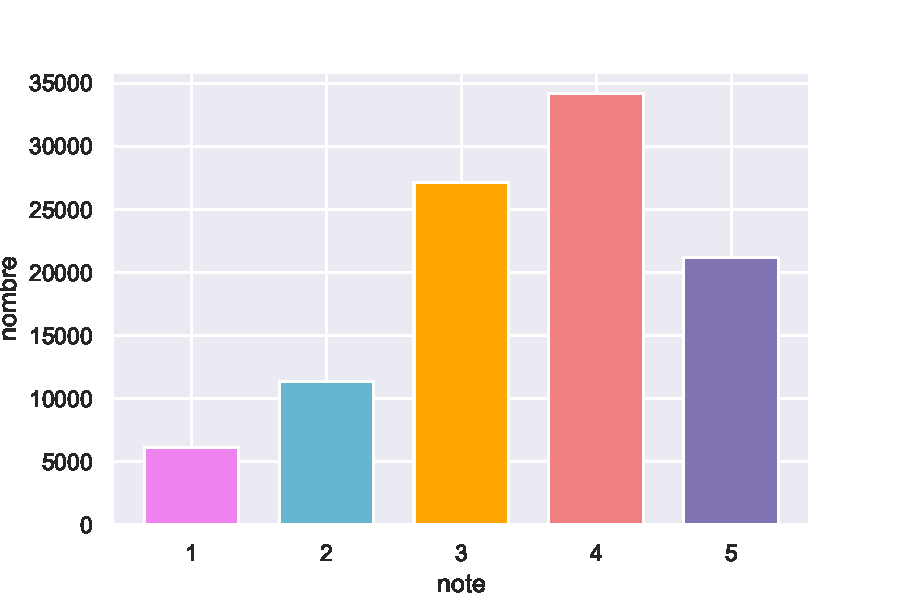
\includegraphics[width=1\linewidth]{./images/distrib_notes.pdf}
  \caption{Ratings distributions.}
  \label{fig:distri_notes}
\end{subfigure}%
\begin{subfigure}{.5\textwidth}
  \centering
  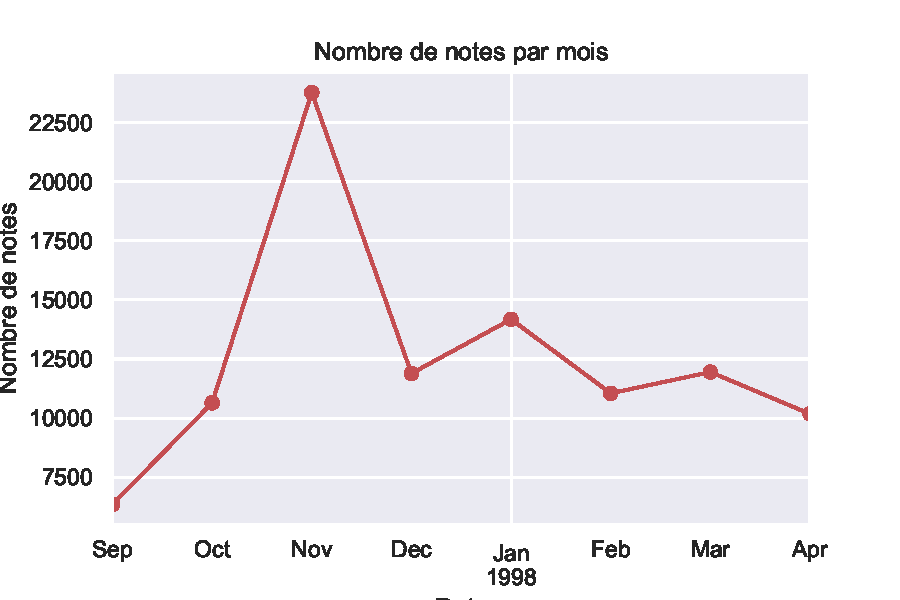
\includegraphics[width=1\linewidth, clip,trim={0cm 0cm 0cm 0.6cm} ]{./images/notes_mois.pdf}
  \caption{Number of ratings per month.}
  \label{fig:mois}
\end{subfigure}
\caption{Graphical representation of some data.}
\label{fig:notes_mois}
\end{figure}

We notice in Figure \ref{fig:distri_notes} that the rating most often put for a movie is $4$. Conversely, the one least put to rate a movie is $1$. Moreover, in Figure \ref{fig:mois}, we notice that it is during the month of November that the most films are noted.
%%%%%%%%%%%%%%%%%%%%%%%%%%%%%%%%%%%%%%%%%%%%%%%%%%%%%%%%%%%%%%%%%%%%%%%%%%%%%%%
%%%%%%%%%%%%%%%%%%%%%%%%%%%%%%%%%%%%%%%%%%%%%%%%%%%%%%%%%%%%%%%%%%%%%%%%%%%%%%%

%%%%%%%%%%%%%%%%%%%%%%%%%%%%%%%%%%%%%%%%%%%%%%%%%%%%%%%%%%%%%%%%%%%%%%%%%%%%%%%
%%%%%%%%%%%%%%%%%%%%%%%%%%%%%%%%%%%%%%%%%%%%%%%%%%%%%%%%%%%%%%%%%%%%%%%%%%%%%%%
\section{Matrix factorisation}
\subsection{Sparse matrix}
Note
$$Y \in \mathbb{R}^{n \times p}$$ the matrix containing user ratings by movies with $n=943$ the number of users and $p=1682$ the number of movies. Each array element $y_{ij}$ correspond to a user rating $i$ of the movie $j$. So, we have:
$$Y=\begin{bmatrix}
5 & 3 & 4 & \dots & 0 & 0 & 0\\
4 & 0 & 0 & \dots & 0 & 0 & 0\\
0 & 0 & 0 & \dots & 0 & 0 & 0\\
  &   &   & \vdots\\
5 & 0 & 0 & \dots & 0 & 0 & 0\\
0 & 0 & 0 & \dots & 0 & 0 & 0\\
0 & 5 & 0 & \dots & 0 & 0 & 0\\
\end{bmatrix}$$

First of all, we can say that the matrix $Y$ contains a lot of null values since users have evaluated at least $20$ movies on all available movies. So it’s a sparse matrix.
However, the null values in the rating matrix does not correspond to a null rating as these are between $1$ and $5$. These zero scores are actually entries that we don’t have.

We study the sparsity of the $Y$ matrix in order to observe this phenomenon. The sparsity of the $Y$ matrix is defined by the ratio of its number of null coefficients to the total number of coefficients. It can also be defined by subtraction of $1$ and the ratio of its number of nonzero coefficients to the total number of coefficients.

\begin{table}[H]
    \centering
    \begin{tabular}{|c|c|c|c|}
    \hline
      nb of nonzero coeff &  nb total coeff & sparsity \\\hline
        100000 & 1586126 & 93.695 \\\hline
    \end{tabular}
    \caption{Results of the sparsity of the matrix $Y$ from \texttt{Python}.}
    \label{tab:sparsity}
\end{table}

Based on the results of the Table \ref{tab:sparsity}, we can say that the $Y$ matrix has a sparsity of about $94\%$. Thus, it will be composed of null values at $94\%$. Let’s visualize this sparsity with a graph.
\begin{figure}[H]
\centering
  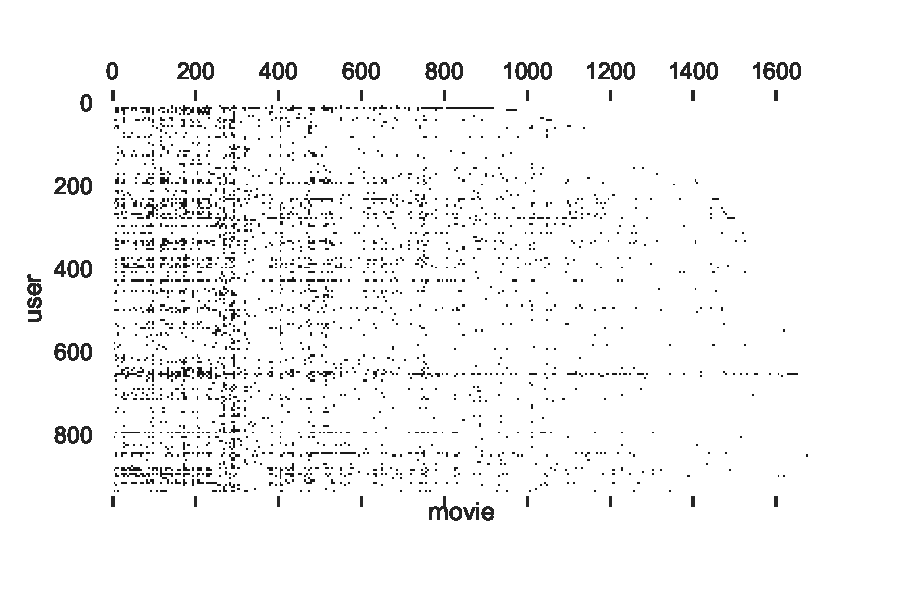
\includegraphics[scale=0.68]{./images/sparse.pdf}
  \caption{Sparsity of the matrix $Y$.}
  \label{fig:sparse_fig}
\end{figure}

In Figure \ref{fig:sparse_fig}, a black square corresponds to a rating assigned by a user for a movie. Since it has many white areas, this means that a lot of user-movie data is incomplete. This seems consistent because each user did not note down all the movie available.

\subsection{Size reduction}
Matrix factorization allows from a large matrix to decompose it as the product of two sub-matrices. This makes it possible to reduce the dimension. In our case, we have:
$$Y \approx U\times V^{\top}.$$.

\begin{figure}[H]
\centering
  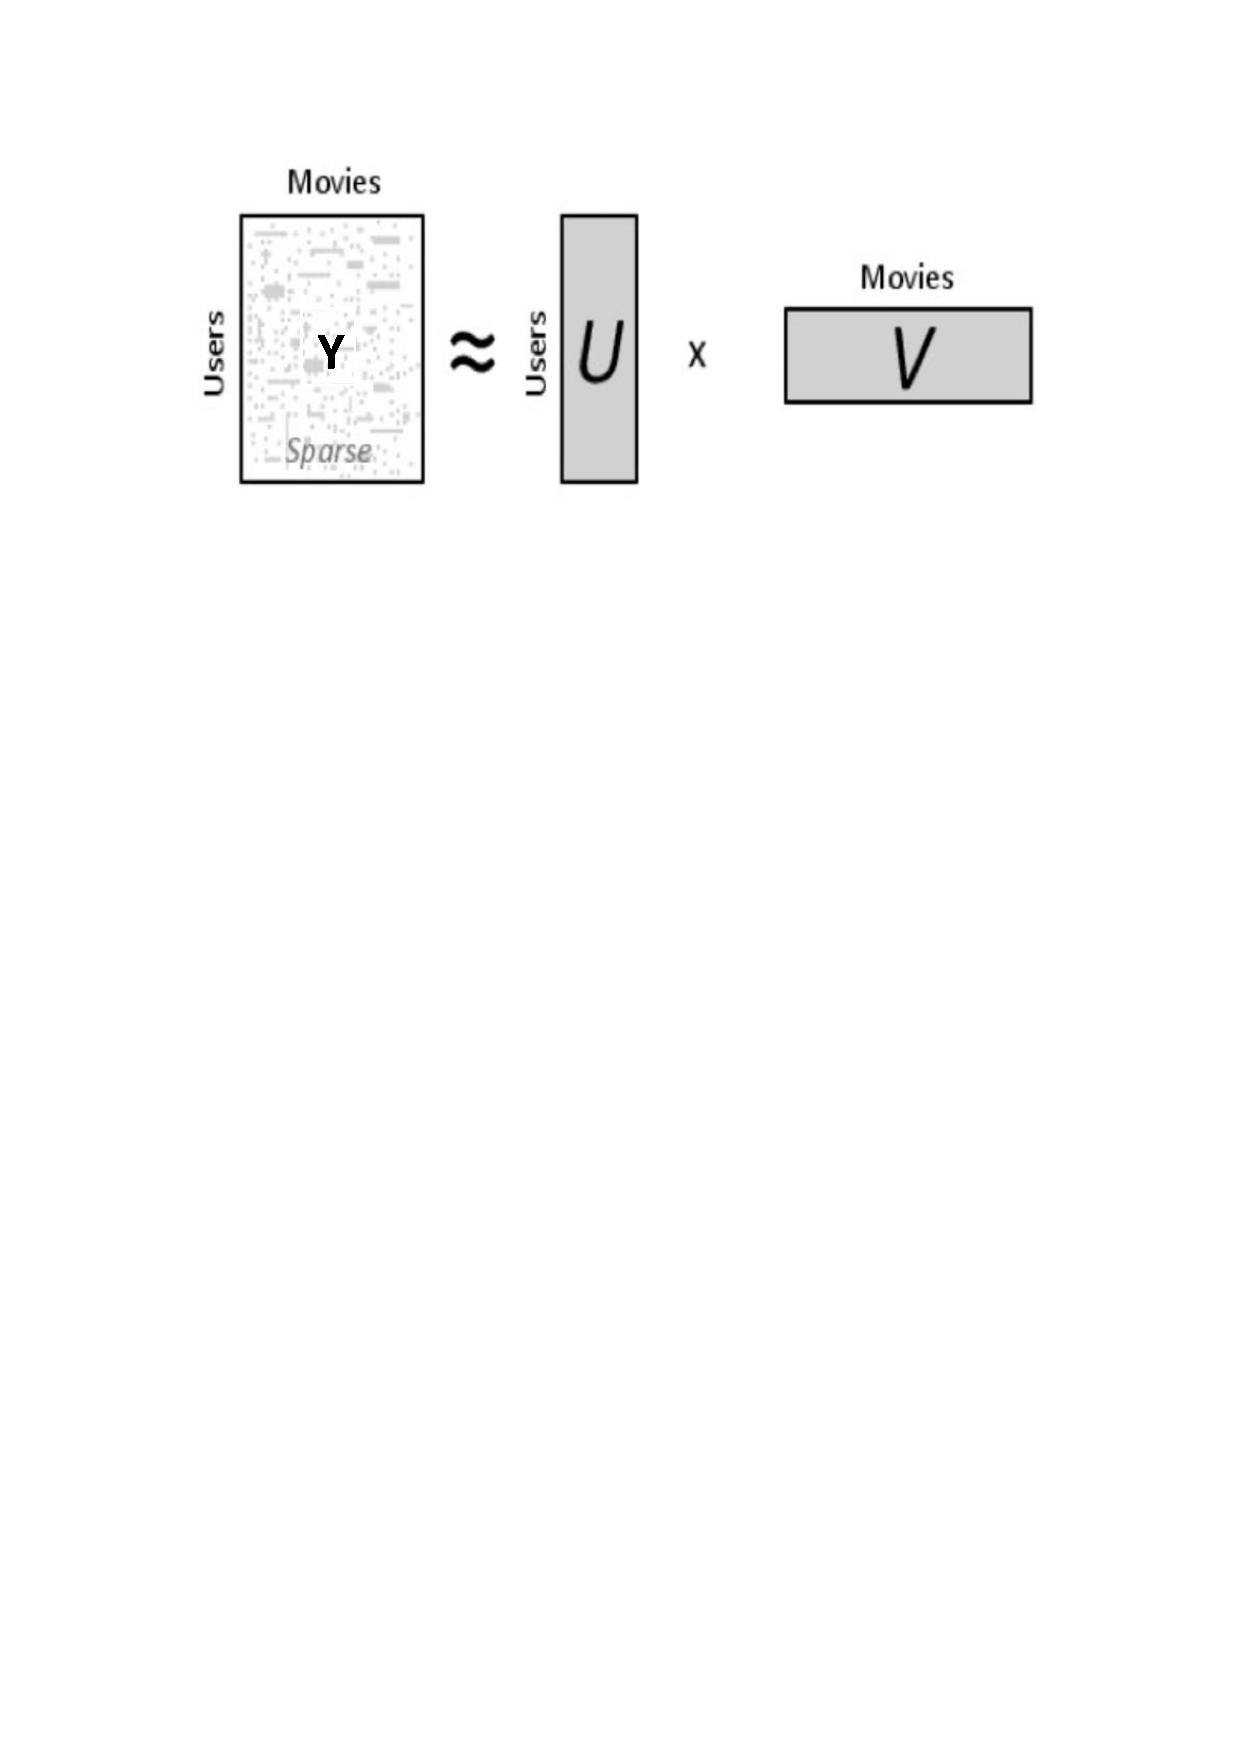
\includegraphics[scale=0.4]{./images/facto.pdf}
  \caption{$Y$-matrix factorisation.}
  \label{fig:facto}
\end{figure}    

In order to know the $U$ and $V$ matrix, we use the reduced singular value decomposition. Thus, we have:

\begin{figure}[H]
\centering
  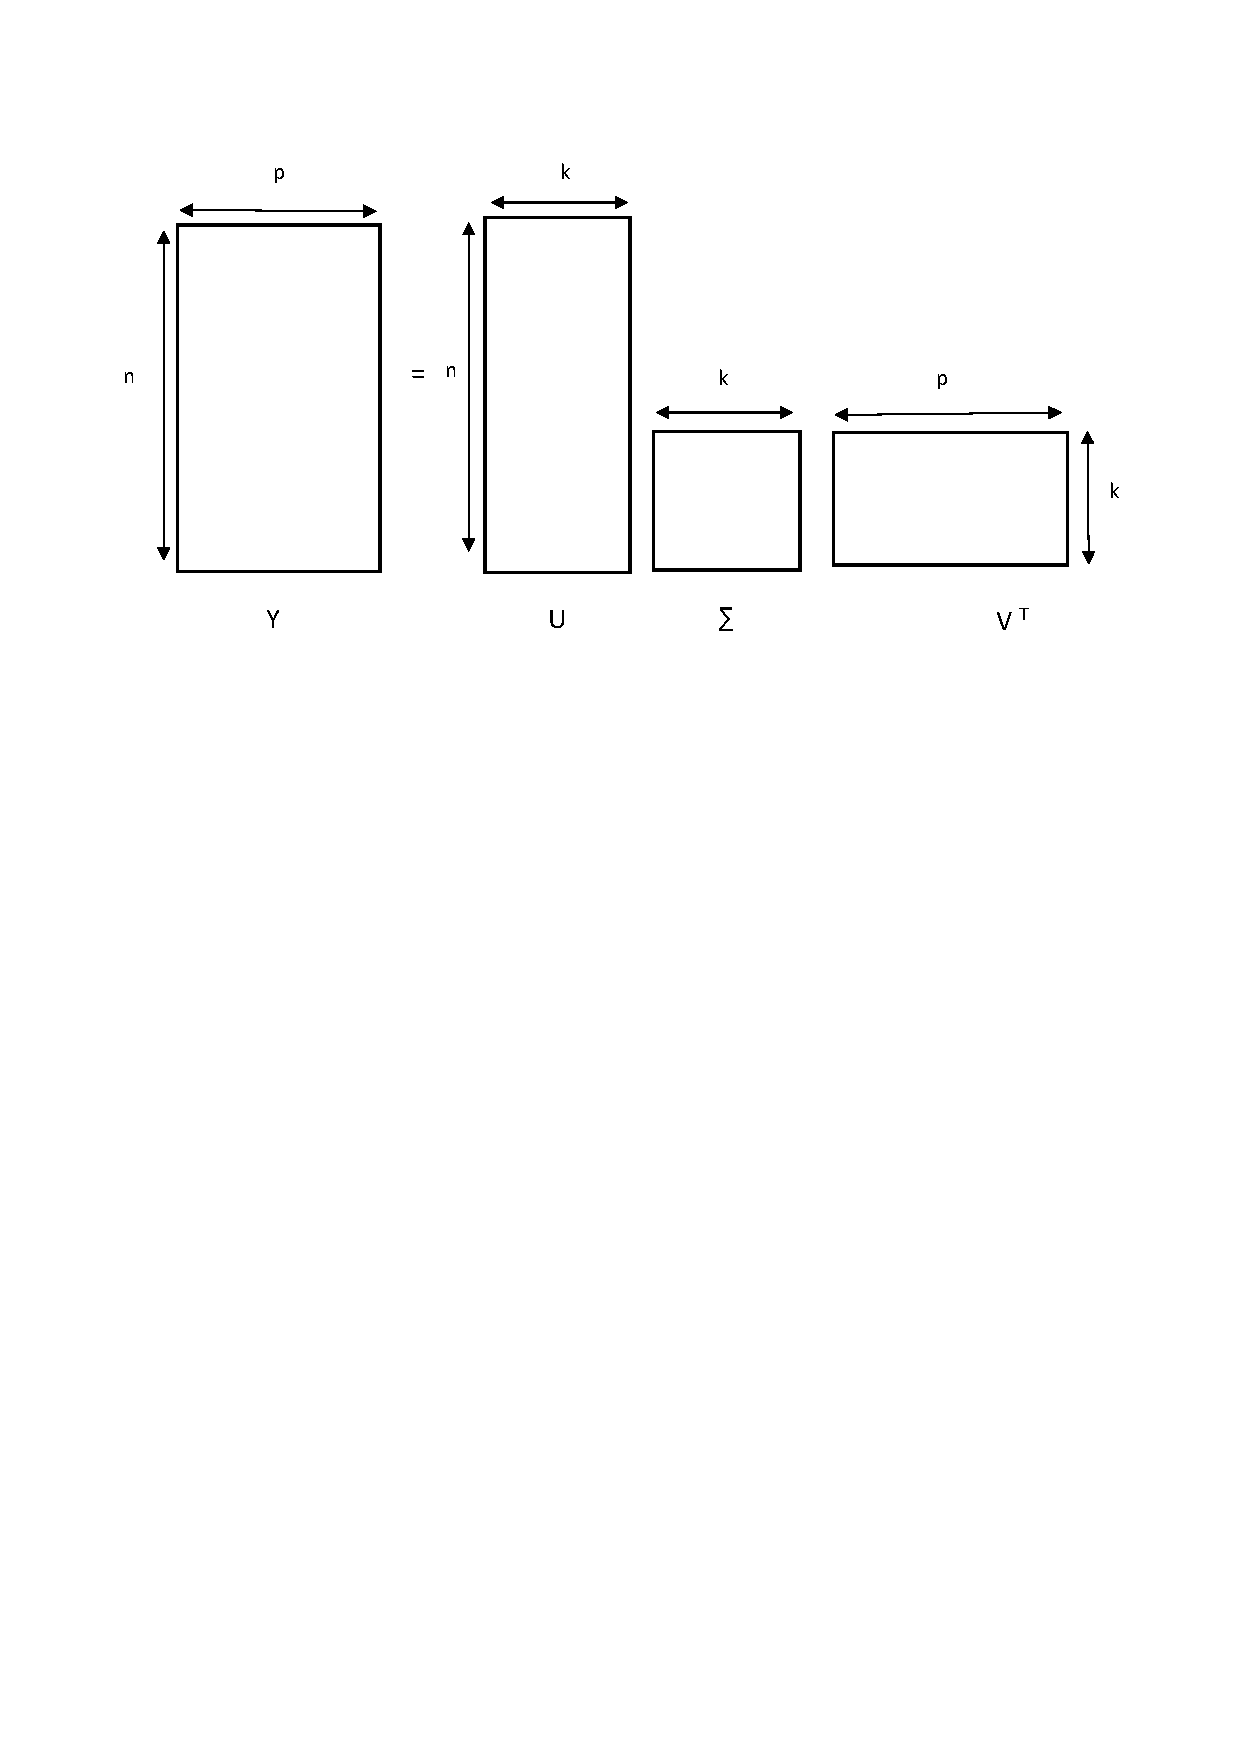
\includegraphics[scale=0.5]{./images/svd.pdf}
  \caption{Reduced SVD.}
  \label{fig:svd}
\end{figure} 

with $n=943$, $k=6$ and $p=1682$.

In order to get an approximation of the rating that a user would give to a movie, we need to learn the $U$ (user matrix) and $V$ (movie matrix) matrix by minimizing a  loss function $L$ and finally performing a matrix multiplication on both.
The prediction of the rating that a user $i$ would give to a movie $j$
is:
\[ \hat{y}_{ij}=u_i v_j^{\top},\]
where $\hat{y}_{ij}$ represents the prediction of the true rating $y_{ij}$.

A quadratic objective function is chosen to minimize the difference between the ratings in our dataset and the predictions made.
Noting the DF dataset, we have:
\begin{align*}
   L&=\sum_{i,j \in DF} (y_{ij} - \hat{y}_{ij})^2 + \lambda\left(\sum_i || u_i ||^2 + \sum_j || v_j ||^2\right) \\
   &=\sum_{i,j \in DF} (y_{ij} - u_i v_j^{\top} )^2 + \lambda\left(\sum_i || u_i ||^2 + \sum_j || v_j ||^2\right) \enspace .
\end{align*}

We calculate the partial derivatives of the loss function $L$. We have:
\begin{align*}
    \dfrac{\partial L }{\partial u_{i_0}}&=\dfrac{\partial}{\partial u_{i_0}}\left[\sum_{i,j \in DF} (y_{ij} - u_i v_j^{\top} )^2 + \lambda\left(\sum_i || u_i ||^2 + \sum_j || v_j ||^2\right)\right]\\
    &=\sum_j \dfrac{\partial}{\partial u_{i_0}}\left[\sum_i (y_{ij} - u_i v_j^{\top} )^2\right] + \lambda \dfrac{\partial}{\partial u_{i_0}} ||u_{i_0} ||^2\\
    &= -2 \sum_j (y_{i_0j} -  u_{i_0} v_{j}^{\top} )v_j + 2\lambda u_{i_0} \enspace ,
\end{align*}

\begin{align*}
    \dfrac{\partial L }{\partial v_{j_0}}&=\dfrac{\partial}{\partial v_{j_0}}\left[\sum_{i,j \in DF} (y_{ij} - u_i v_j^{\top} )^2 + \lambda\left(\sum_i || u_i ||^2 + \sum_j || v_j ||^2\right)\right]\\
    &=\sum_i \dfrac{\partial}{\partial v_{j_0}}\left[\sum_j (y_{ij} - u_i v_j^{\top} )^2\right] + \lambda \dfrac{\partial}{\partial v_{j_0}} ||v_{j_0} ||^2\\
    &= -2 \sum_i (y_{ij_0} -  u_i v_{j_0}^{\top} )u_i + 2\lambda v_{j_0} \enspace .
\end{align*}
%%%%%%%%%%%%%%%%%%%%%%%%%%%%%%%%%%%%%%%%%%%%%%%%%%%%%%%%%%%%%%%%%%%%%%%%%%%%%%%
%%%%%%%%%%%%%%%%%%%%%%%%%%%%%%%%%%%%%%%%%%%%%%%%%%%%%%%%%%%%%%%%%%%%%%%%%%%%%%%

%%%%%%%%%%%%%%%%%%%%%%%%%%%%%%%%%%%%%%%%%%%%%%%%%%%%%%%%%%%%%%%%%%%%%%%%%%%%%%%
%%%%%%%%%%%%%%%%%%%%%%%%%%%%%%%%%%%%%%%%%%%%%%%%%%%%%%%%%%%%%%%%%%%%%%%%%%%%%%%
\section*{Conclusion}
To sum up all of it, we have studied the dataset MovieLens (100k) in order to try to predict the ratings that a user would give to a movie they haven't seen yet.
We were able to see how to use the matrix factorization to make it possible to reduce the dimension of the studied matrix.
But also, the sparsity of a matrix in order to know the number of null ratings (which in fact correspond to missing data).

%%%%%%%%%%%%%%%%%%%%%%%%%%%%%%%%%%%%%%%%%%%%%%%%%%%%%%%%%%%%%%%%%%%%%%%%%%%%%%%
%%%%%%%%%%%%%%%%%%%%%%%%%%%%%%%%%%%%%%%%%%%%%%%%%%%%%%%%%%%%%%%%%%%%%%%%%%%%%%%

%%%%%%%%%%%%%%%%%%%%%%%%%%%%%%%%%%%%%%%%%%%%%%%%%%%%%%%%%%%%%%%%%%%%%%%%%%%%%%%
%%%%%%%%%%%%%%%%%%%%%%%%%%%%%%%%%%%%%%%%%%%%%%%%%%%%%%%%%%%%%%%%%%%%%%%%%%%%%%%
\nocite{*}
\printbibliography
%%%%%%%%%%%%%%%%%%%%%%%%%%%%%%%%%%%%%%%%%%%%%%%%%%%%%%%%%%%%%%%%%%%%%%%%%%%%%%%
%%%%%%%%%%%%%%%%%%%%%%%%%%%%%%%%%%%%%%%%%%%%%%%%%%%%%%%%%%%%%%%%%%%%%%%%%%%%%%%

\end{document}

%%%%%%%%%%%%%%%%%%%%%%%%%%%%%%%%%%%%%%%%%%%%%%%%%%%%%%%%%%%%%%%%%%%%%%%%%%%%%%%
%%%%%%%%%%%%%%%%%%%%%%%%%%%%%%%%%%%%%%%%%%%%%%%%%%%%%%%%%%%%%%%%%%%%%%%%%%%%%%%

%%%%%%%%%%%%%%%%%%%%%%%%%%%%%%%%%%%%%%%%%%%%%%%%%%%%%%%%%%%%%%%%%%%%%%%%%%%%%%%
%%%%%%%%%%%%%%%%%%%%%%%%%%%%%%%%%%%%%%%%%%%%%%%%%%%%%%%%%%%%%%%%%%%%%%%%%%%%%%%
\nocite{*}
\printbibliography
%%%%%%%%%%%%%%%%%%%%%%%%%%%%%%%%%%%%%%%%%%%%%%%%%%%%%%%%%%%%%%%%%%%%%%%%%%%%%%%
%%%%%%%%%%%%%%%%%%%%%%%%%%%%%%%%%%%%%%%%%%%%%%%%%%%%%%%%%%%%%%%%%%%%%%%%%%%%%%%

\end{document}